
\MTtitle{Recolección de información de Internet} 

%-------------------------------Web Scraping----------------------------------------------%

\section{Web Scraping}

La recopilación de datos de Internet es una técnica que se realiza de manera manual, sin embargo 
el \textit{Web Scraping} es el conjunto de técnicas utilizadas para obtener de manera automática información de 
un sitio web \citep{CTWebScraping}. 
%El objetivo del Web Scraping es buscar cierto tipo de información definida y agregarla a nuevas páginas web. 
\\
El \textit{Web scraping} accede a las páginas web, encuentra los elementos de datos especificados en la 
página, los extrae y transforma en diferentes formatos si es necesario, finalmente, guarda 
la información como un conjunto de datos estructurado\footnote{Un conjunto de datos estructurado permite recolectar 
varios valores simultáneamente.}. Los investigadores limpian y organizan el contenido para analizar la información.

%------------------------Técnicas de Web Scraping----------------------------------------------%

\subsection{Técnicas de web scraping}

Algunas de las técnicas que nos proporciona el \textit{Web scraping} son\citep{CTTechniques}:

\begin{itemize}

    \item \textbf{Copiar y pegar}: Realiza el método recolección copiar y pegar la información, 
    sin embargo es una técnica propensa a errores

    \item \textbf{Uso de expresiones regulares}: Es una técnica que se puede utilizar para obtener la información 
    de las páginas web son las expresiones regulares, aunque comúnmente no se recomienda utilizarlas para parsear el formato HTML

    \item \textbf{Reconocimiento de anotaciones semánticas}: Las páginas que contienen metadatos, 
    marcas semánticas o explicaciones adicionales que se pueden usar para encontrar fragmentos de datos específicos

    \item \textbf{Parsers de HTML}: Algunos lenguajes, como XQuery y HTQL pueden ser utilizados para parsear documentos, recuperar 
    y transformar el contenido de documentos HTML

\end{itemize}

En el presente trabajo se hará uso de la técnicas \textbf{Uso de expresiones regulares}.\\
La Figura \textbf{\ref{fig:procesos}} muestra los procesos.

\begin{figure}[H]
    \centering
    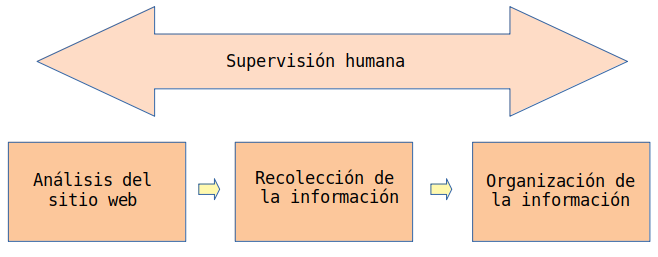
\includegraphics[scale=.35]{imagenes/Capitulo3/procesos}
    \caption{Etapas del proceso de \textit{Web scraping}.}
    \label{fig:procesos}
  \end{figure}
  
%--------------------------------Crawler---------------------------------------------%

\section{Crawler}

Un \textit{Crawler}  es una herramienta la cual analiza sitios web, permitiendo recolectar 
las páginas web para así posteriormente extraer la información que contengan \citep{CTCrawler}. Un crawler también 
conocido como como robot o spider, es un sistema para la descarga masiva de páginas web. Son uno de 
los componentes principales de los motores de búsqueda web, los sistemas que reúnen un conjunto de 
páginas web, las indexan y permiten a los usuarios realizar consultas contra el índice y encontrar las 
sitios que coincidan con las consultas.

%--------------------------------Python---------------------------------------------%

\section{Python}
\textit{Python}\footnote{http://www.python.org/} un lenguaje de programación creado en 1991, se ha convertido en uno de los más 
importantes lenguajes de programación para la ciencia de datos, el aprendizaje automático y el desarrollo general de software en 
el mundo académico y la industria. 
En los últimos años, el soporte mejorado de Python para bibliotecas (como pandas y scikit-learn) lo ha convertido en una opción popular 
para las tareas de análisis de datos. Combinado con la solidez general de Python para la ingeniería de software de propósito general, 
es una excelente opción como idioma principal para crear aplicaciones de datos \citep{CTPython}.

%--------------------------------Scrapy---------------------------------------------%

\subsection{Scrapy}
\textit{Scrapy} es un \textit{framework} para rastrear sitios web y extraer datos estructurados que pueden utilizarse para una amplia 
gama de aplicaciones útiles, como la extracción de datos, el procesamiento de información o el archivo histórico.
A pesar de que Scrapy fue diseñado originalmente para el \textit{Web scraping}, también se puede usar para extraer datos mediante 
API (como los Servicios web de Amazon Associates) \citep{CTScrapy}.\\

La arquitectura del proyecto Scrapy se basa en arañas, que son rastreadores independientes que reciben un conjunto de instrucciones,
hace que sea más fácil construir y escalar grandes proyectos de \textit{Crawler} al permitir que los desarrolladores reutilicen su 
código. Scrapy también proporciona un una terminal de rastreo web, que los desarrolladores pueden usar para probar sus suposiciones 
sobre el comportamiento de un sitio.
